\documentclass{beamer}
\usetheme[pageofpages=of,% String used between the current page and the
                         % total page count.
          bullet=circle,% Use circles instead of squares for bullets.
          titleline=true,% Show a line below the frame title.
          alternativetitlepage=true,% Use the fancy title page.
       %   titlepagelogo=logo-polito,% Logo for the first page.
       %   watermark=watermark-polito,% Watermark used in every page.
       %   watermarkheight=100px,% Height of the watermark.
       %   watermarkheightmult=4,% The watermark image is 4 times bigger
                                % than watermarkheight.
          ]{Torino}

\author{Brendon J. Brewer}
\title{Introduction to Nested Sampling}
\institute{Department of Statistics, The University of Auckland}
\date{{\color{blue} https://www.stat.auckland.ac.nz/\~{ }brewer}\\
\vspace{10pt}
{\color{blue} @brendonbrewer}}

\usepackage{dsfont}
\usepackage{minted}

\begin{document}

\begin{frame}[t,plain]
\titlepage
\end{frame}

\begin{frame}[t]{Transit Example}
\begin{figure}
\includegraphics[scale=0.4]{figures/transit_data.pdf}
\end{figure}
\end{frame}



\begin{frame}[t]{Related to the transit example...}
\begin{itemize}
\item Realistic exoplanet transits
\item Finding emission/absorption lines in spectra
\item Finding stars/galaxies in an image
\item All ``curve fitting''
\end{itemize}
\end{frame}


\begin{frame}[t]{Transit Example: The Truth}
The red curve was:
\begin{eqnarray*}
\mu(t) &=& \left\{
\begin{array}{lr}
10, & 2.5 \leq t \leq 4.5\\
5,  & \textnormal{otherwise}.
\end{array}
\right.
\end{eqnarray*}

\begin{figure}
\includegraphics[scale=0.3]{figures/transit_data.pdf}
\end{figure}
\end{frame}

\begin{frame}[fragile, t]{Transit Example: The Truth}
The red curve was:
\begin{eqnarray*}
\mu(t) &=& \left\{
\begin{array}{lr}
10, & 2.5 \leq t \leq 4.5\\
5,  & \textnormal{otherwise}.
\end{array}
\right.
\end{eqnarray*}

and the noise was added like this:
\begin{minted}[mathescape,
               numbersep=5pt,
               gobble=2,
               frame=lines,
               framesep=2mm]{python}
  # Add noise
  sig = 1.
  y += sig*rng.randn(y.size)
\end{minted}
\end{frame}

\begin{frame}[fragile, t]{Transit Example: Inference}
Let's fit the data with this model:
\begin{eqnarray*}
\mu(t) &=& \left\{
\begin{array}{lr}
A, & (t_c - w/2) \leq t \leq (t_c + w/2)\\
A-b,  & \textnormal{otherwise}.
\end{array}
\right.
\end{eqnarray*}

We don't know $A$, $b$, $t_c$, and $w$. But we do know the data $D$.
\end{frame}



\begin{frame}[fragile, t]{Transit Example: Parameters}
We don't know $A$, $b$, $t_c$, and $w$.
These are our unknown parameters. Let's find the posterior.

\begin{eqnarray*}
p(A, b, t_c, w | D) &=& \frac{p(A, b, t_c, w)p(D | A, b, t_c, w)}{p(D)}
\end{eqnarray*}

and the marginal likelihood

\begin{eqnarray*}
p(D) &=& \int p(A, b, t_c, w)p(D | A, b, t_c, w) \, dA \, db \, dt_c \, dw
\end{eqnarray*}

\end{frame}

\begin{frame}[t]{Uniform Priors}
For all four parameters:

\begin{eqnarray*}
A &\sim& U(-100, 100)\\
b &\sim& U(0, 10)\\
t_c &\sim& U(t_{\rm min}, t_{\rm max})\\
w &\sim& U(0, t_{\rm max} - t_{\rm min})
\end{eqnarray*}

Where $t_{\rm min}$ and $t_{\rm max}$ give the time range of the dataset.
Question: is this legitimate? Are we using the data to set our priors?

\end{frame}


\begin{frame}[t]{Sampling Distribution / Likelihood}
Let's assume ``gaussian noise'':

\begin{eqnarray*}
p(y_i | A, b, t_c, w) &=& \prod_{i=1}^N \frac{1}{\sigma_i\sqrt{2\pi}}
\exp\left[
-\frac{1}{2\sigma_i^2}\left(y_i - m(t_i; A, b, t_c, w)\right)^2
\right].
\end{eqnarray*}
or more concisely:
\begin{eqnarray*}
y_i | A, b, t_c, w \sim \mathcal{N}\left(m(t_i; A, b, t_c, w), \sigma_i^2\right).
\end{eqnarray*}

\end{frame}



\begin{frame}[t]{Nested Sampling}
Nested Sampling is a Monte Carlo method (not necessarily MCMC) that was
introduced by John Skilling in 2004.\\
\vspace{20pt}
It is very popular in astrophysics and has some unique strengths.
\end{frame}


\begin{frame}[t]{Marginal Likelihood}
The {\bf marginal likelihood} is useful for ``model selection''. Consider
two models: $M_1$ with parameters $\theta_1$, $M_2$ with parameters $\theta_2$.
The marginal likelihoods are:
\begin{eqnarray*}
p(D | M_1) &=& \int p(\theta_1 | M_1) p(D | \theta_1, M_1) \, d\theta_1\\
p(D | M_2) &=& \int p(\theta_2 | M_2) p(D | \theta_2, M_2) \, d\theta_2
\end{eqnarray*}

These are the normalising constants of the posteriors, within each model.
\end{frame}


\begin{frame}[t]{Bayesian Model Selection}
If you have the marginal likelihoods, it's easy:

\begin{eqnarray*}
\frac{P(M_1 | D)}{P(M_2 | D)} &=& \frac{P(M_1)}{P(M_2)}
\times \frac{P(D | M_1)}{P(D | M_2)}.
\end{eqnarray*}

\begin{eqnarray*}
\textnormal{(posterior odds)} = \textnormal{(prior odds)} \times \textnormal{(bayes factor)}
\end{eqnarray*}

\end{frame}


\begin{frame}[t]{Challenging features}
Another motivation: standard MCMC methods can get stuck in the following
situations:
\begin{center}
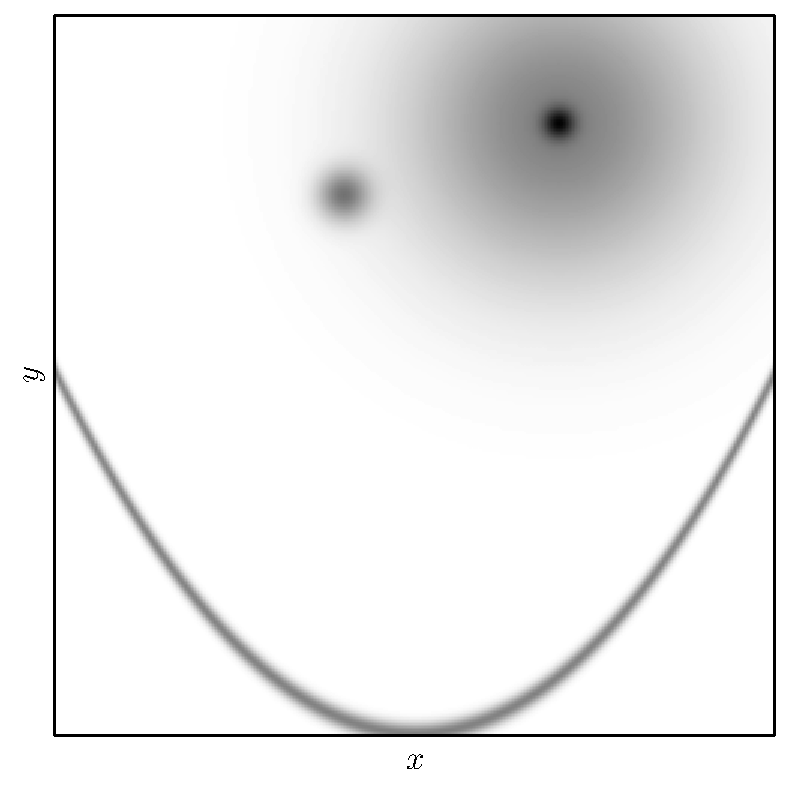
\includegraphics[scale=0.4]{figures/challenges.pdf}
\end{center}
\end{frame}

\begin{frame}{Nested Sampling}
Nested Sampling was built to estimate the marginal likelihood.

But it can also be used to generate posterior samples, and it can potentially
work on harder problems where standard MCMC methods get stuck.
\end{frame}

\begin{frame}[t]{Notation}
When discussing Nested Sampling, we use different symbols:
\begin{eqnarray*}
p(D | M_1) &=& \int p(\theta_1 | M_1) p(D | \theta_1, M_1) \, d\theta_1\\
\end{eqnarray*}
becomes
\begin{eqnarray*}
Z &=& \int \pi(\theta) L(\theta) \, d\theta.
\end{eqnarray*}

$Z$ = marginal likelihood, $L(\theta)$ = likelihood function, $\pi(\theta)$ = prior
distribution.
\end{frame}


\begin{frame}[t]{Nested Sampling}
Imagine we had an easy 1-D problem, with a Uniform(0, 1) prior, and a likelihood
that was strictly decreasing.

\begin{center}
\begin{figure}
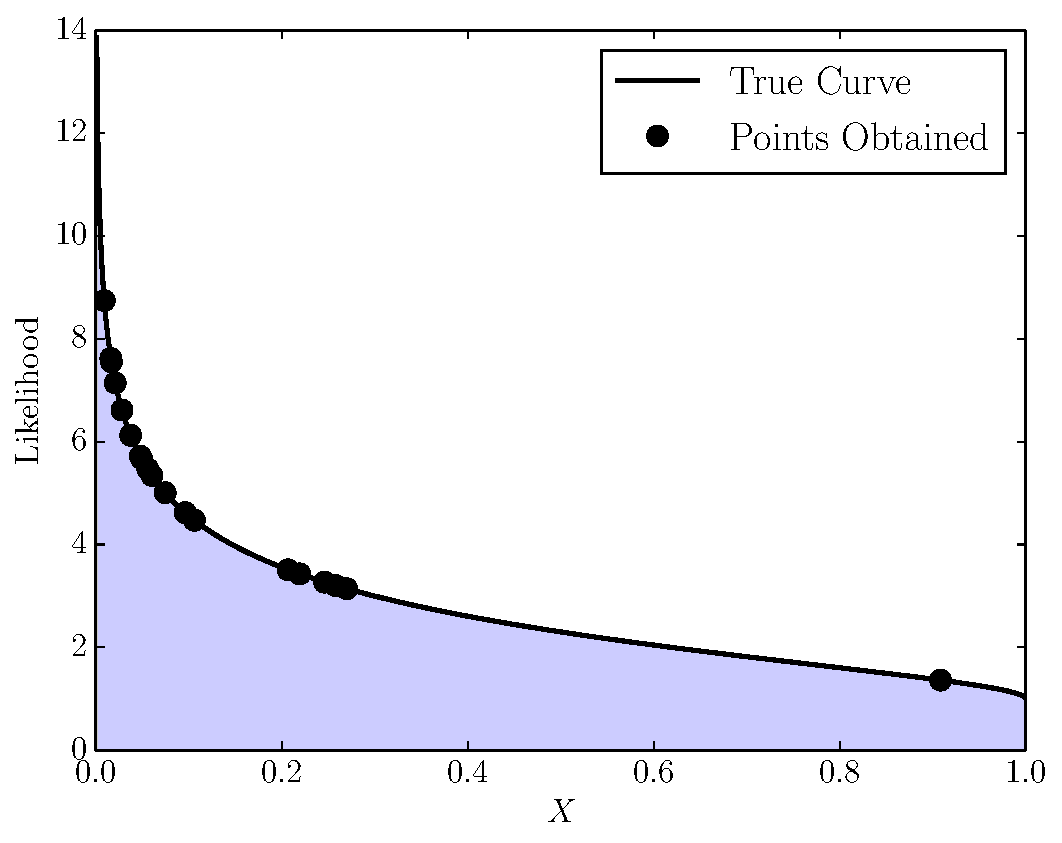
\includegraphics[scale=0.35]{figures/nested1.pdf}
\caption{Likelihood function with area Z.}
\end{figure}
\end{center}

\end{frame}


\begin{frame}[t]{Nested Sampling}
The key idea of Nested Sampling: Our high dimensional problem can be mapped
onto the easy 1-D problem. Figure from Skilling (2006):

\begin{figure}
\begin{center}
\includegraphics[scale=0.3]{figures/ns.png}
\end{center}
\end{figure}

\end{frame}

\begin{frame}{Nested Sampling $X$}
\vspace{-20pt}
Define
\begin{eqnarray*}
X(L^*) = \int \pi(\theta) \mathds{1}\left(L(\theta) > L^*\right)\, d\theta
\end{eqnarray*}

\vspace{10pt}

$X$ is the {\bf amount of prior probability} with likelihood greater than $L^*$.
Loosely, $X$ is the {\bf volume} with likelihood above $L^*$.\\
Higher $L^* \Leftrightarrow$ lower volume.
\end{frame}
\begin{frame}{Numerical Integration}
If we had some points with likelihoods $L_i$, and we knew the corresponding
$X$-values, we could approximate the integral numerically, using the
trapezoidal rule or something similar.
%\begin{center}
%\includegraphics[scale=0.25,clip=true,angle=0]{Patricio/SampleLike2.pdf}
%\end{center}
\end{frame}
%######################################%##########################################################################################################################################
\begin{frame}{Nested Sampling Procedure}
This procedure gives us the likelihood values. \\

\begin{itemize}
	\item Sample $\theta=\{\theta_{1}, \ldots , \theta_{N}\}$ from the prior $\pi(\theta)$.
	\item Find the point $\theta_k$ with the worst
likelihood, and let $L^*$ be its likelihood.
	\item Replace $\theta_{k}$ with a new point from $\pi(\theta)$ but restricted to the region where $L(\theta)>L^*$.
\end{itemize}

Repeat the last two steps many times.
The \textit{discarded points} (the worst one at each iteration) are the output.
\end{frame}


\begin{frame}[t]{Generating the new point}
We need a new point from $\pi(\theta)$ but restricted to the region where $L(\theta)>L^*$. The point being replaced has the worst likelihood, so
{\bf all the other points satisfy the constraint!}
\vspace{20pt}

So we can use one of the other points to initialise an MCMC run, trying to
sample the prior, but rejecting any proposal with likelihood below $L^*$.
See code.
\end{frame}

\begin{frame}[t]{Generating the new point}
There are alternative versions of NS available, such as {\bf MultiNest}, that
use different methods (not MCMC) to generate the new point.\\
\vspace{20pt}

I also have a version of NS called {\bf Diffusive Nested Sampling}, which is
a better way of doing NS when using MCMC. I'm happy to discuss it offline.
\end{frame}


\begin{frame}[t]{Nested Sampling Procedure}
Nested Sampling gives us a sequence of points with increasing likelihoods,
but we need to somehow know their $X$-values!
\end{frame}

\begin{frame}[t]{Estimating the $X$ values}
Consider the simple one-dimensional problem with Uniform(0, 1) prior.\\

\vspace{20pt}
When we generate $N$ points from the prior, the distribution for the $X$-value
of the worst point is Beta$(N, 1)$. So we can use a draw from Beta$(N,1)$ as
a guess of the $X$ value.
\end{frame}

\begin{frame}[t]{Estimating the $X$ values}
Each iteration, the worst point should reduce the volume by a factor that has
a Beta$(N, 1)$ distribution. So we can do this:
\begin{eqnarray*}
X_1 &=& t_1\\
X_2 &=& t_2X_1\\
X_3 &=& t_3X_2\\
\end{eqnarray*}

and so on, where $t_i \sim $Beta$(N,1)$. Alternatively, we can use a simple
approximation.
\end{frame}

%##########################################################################################################################################
\begin{frame}[t]{Deterministic Approximation}
\begin{figure}
\centering
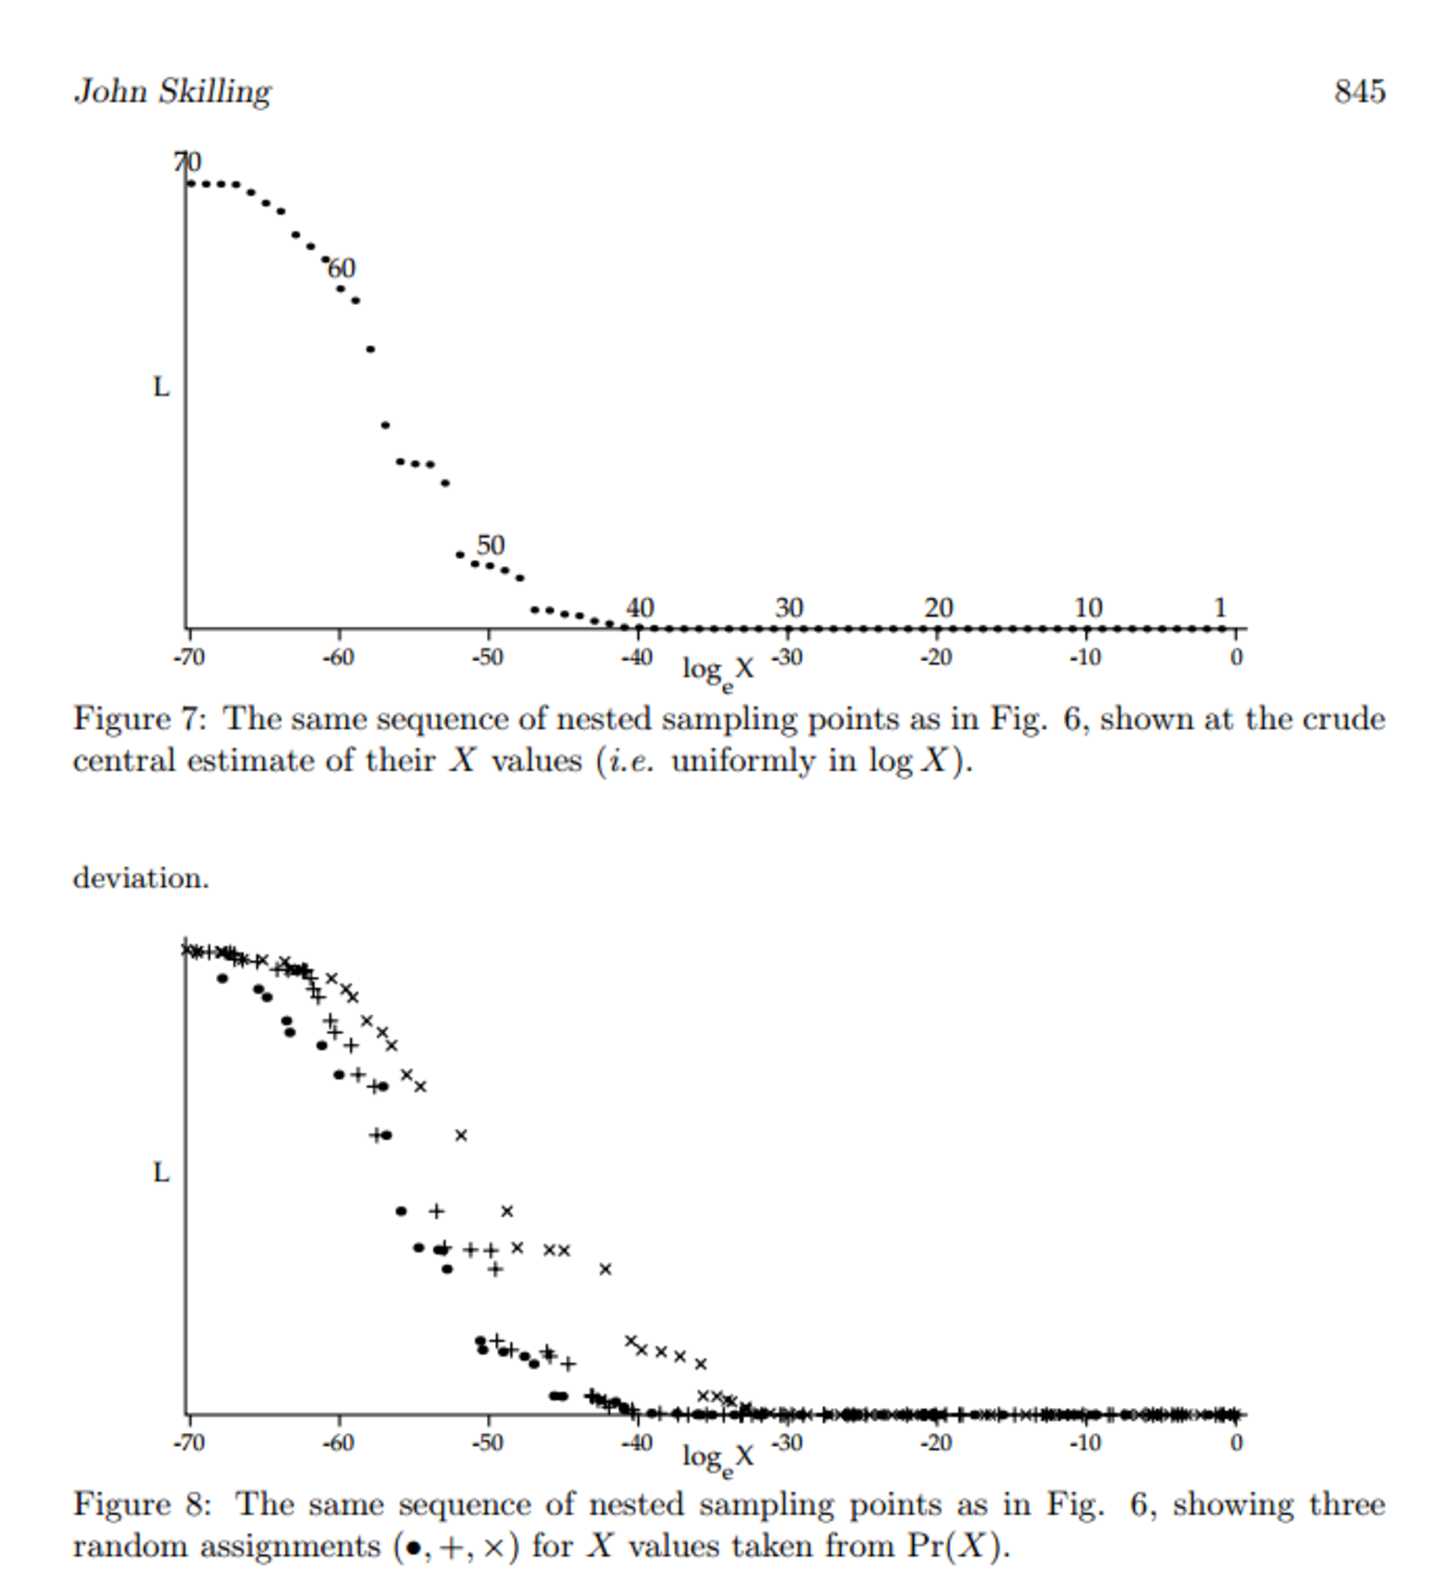
\includegraphics[scale=0.25]{figures/deterministic.pdf}
\caption{Deterministic approximation. Each iteration reduces
the volume by a factor $\approx e^{-1/N}$. e.g. if $N=5$, the worst likelihood
accounts for about 1/5th of the remaining prior volume.}
\end{figure}
\end{frame}

\begin{frame}

\begin{figure}
\centering
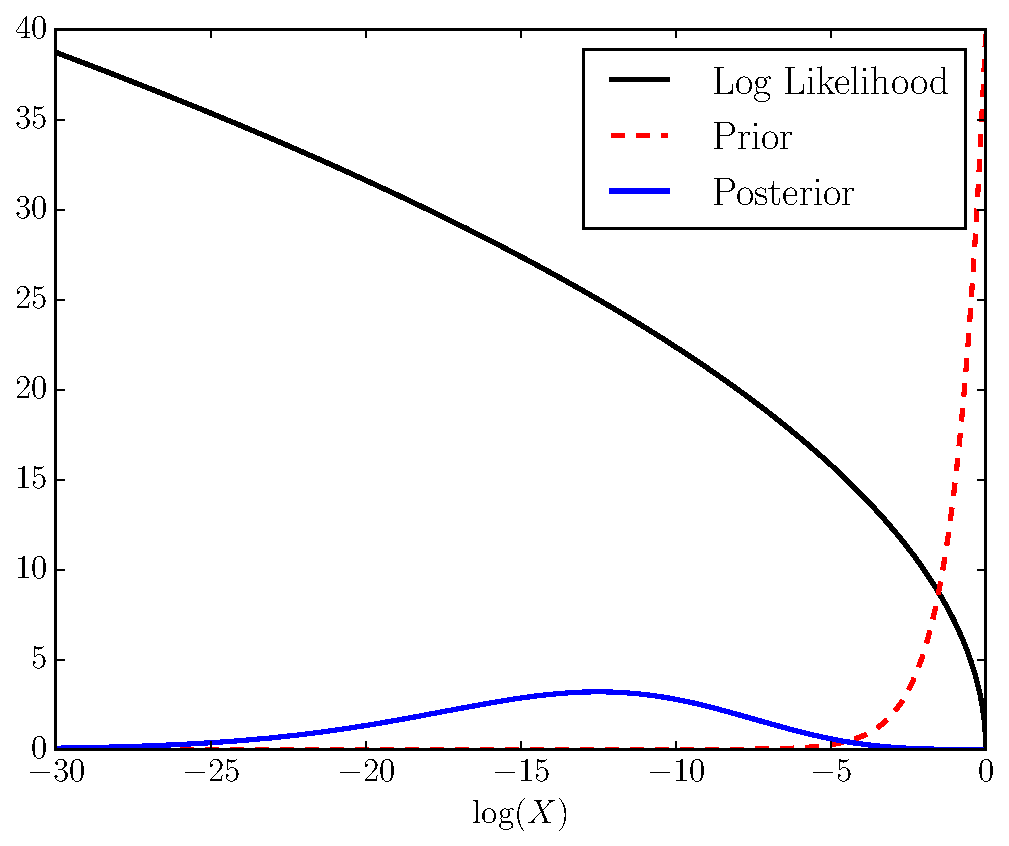
\includegraphics[scale=0.35]{figures/nested2.pdf}
\end{figure}
\end{frame}


\begin{frame}[t]{Posterior Distribution from Nested Sampling}
The posterior sample can be obtained by assigning weights $W_j$ to the
discarded points:
\begin{align*}
W_{j} = \frac{L_{j} w_{j}}{Z} 
\end{align*}
where $w_{j}=X_{j-1} - X_{j+1}$ is the ``prior weight/width'' associated with the
point. The ``effective sample size'' is given by
\begin{align*}
ESS = \exp \left( - \sum_{j=1}^{m} W_j \log W_j \right)
\end{align*}

\end{frame}

\begin{frame}[t]{Information}
NS can also calculate the {\bf information}, also known as the Kullback-Liebler
divergence from the prior to the posterior.

\begin{eqnarray*}
\mathcal{H} &=& \int p(\theta | D) \log\left[\frac{p(\theta | D)}{p(\theta)}\right]
\, d\theta\\
&\approx& \log\left(
\frac{\textnormal{volume of prior}}{\textnormal{volume of posterior}}
\right)
\end{eqnarray*}
\end{frame}

\begin{frame}[t]{Nested Sampling Code}
I have written a basic implementation of Nested Sampling in Python. Let's
use it on the transit problem.

\end{frame}

\begin{frame}[t]{Nested Sampling Plots}
\vspace{-10pt}
%\begin{center}
%\includegraphics[scale=0.32]{ns.pdf}
%\end{center}

\end{frame}

\begin{frame}[t]{Nested Sampling Plots}
A necessary but not sufficient condition for everything being okay is that you
see the entire peak in the posterior weights.\\

\vspace{20pt}

If it's not there, you haven't done enough NS iterations. i.e. your parameter
values have lower likelihoods than what is typical of the posterior distribution.
\end{frame}

\begin{frame}[t]{Nested Sampling Plots}
The shape of the log$(L)$ vs. log$(X)$ plot is also informative: if it is
straight for a long time, or concave up at some point, your problem contains
a phase transition, and it's a good thing you used Nested Sampling!
\end{frame}



\end{document}

